\chapter{Theorical foundations}
In this chapter we will explain the necessary background that is used throughout the thesis. In the following we will introduce the theoretical foundations of compressed sensing and some of the problems one faces when dealing with it. Deep Learning will also be intriudced along with convolutional neural networks which will be dicussed in more detail.  

\section{Compressed Sensing}

Compressed sensing is mathematical theory that deals with the problem of recovering a signal from a small number of measurements, the number of measurements is less than the minimun number of samples defined by Shanon-Nyquist theorem (sampling acquisition must be done at least twice the highest frequency in the signal). For many applications, imaging and video, the sampling rate specified by Nyquist might end up being very large that the amount of samples that have to be compressed and transmitted increases the complexity of the system and makes it costly. Compressed sensing contradicts the previous staments since it claims that a signal may be recovered with lesser samples or measurements than conventional approaches. That is possible because it proposes a generalization of a linear mapping paired with optimization in order do the sampling and recovery process at notably inferior rates than that imposed by Nyquist rate. CS justification is based on two principles: sparcity of the signal, and incoherence which refers to sampling/sensing representation, both terms will be further discussed. In addition to that, CS tries to overcome two of the major incapabilities of sample-compress schemes: First, the number of samples or measurements is cosiderably reduced. Second, the compression stage occurs inside the sensor and therefore there is no need to add extra encoding computation.

\subsection{Sparsity of a signal}
The mathematical formulation of sparcity is defined as follows: a signal $\mathbf{x \in R^N}$ (for instance $n$-pixels of an image) is interpreted in terms of its basis representation as a linear combination of the orthonormal basis $\{\psi\}_{i=1}^{N}$ and coefficients $\mathbf{\alpha}$ as  
\begin{equation} \label{eq:signal}
\hspace{3em} \hspace{3em} x = \sum\limits_{i=1}^N \alpha_{i} \psi_{i} \hspace{3em} or \hspace{3em} \mathbf{x = \Psi \alpha}
\end{equation} 

CS takes advantage of the certainty that plentiful natural signals are sparse or compressible when stated in a condensed representaion. For example, images are easily compressed using the discrete cosine transform (DCT) and wavelet bases \cite{mallat1999wavelet}. Namely, a signal is said to be compressible or k-sparse if there exists a conevenient basis $\psi$ for which $\mathbf{x}$ is a linear combination of only $K$ basis vectors, obeying $K \ll N$. That means, only $K$ elements of $\alpha$ present in \ref{eq:signal} are nonzero. 

\subsection{Incoherence}
Measurements in CS are obtained by using a linear operator that takes $M < N$ inner products between $\mathbf{x}$ and a set of vectors $\{\phi\}_{i=1}^{M}$. \begin{figure}[tb] 
\centering 
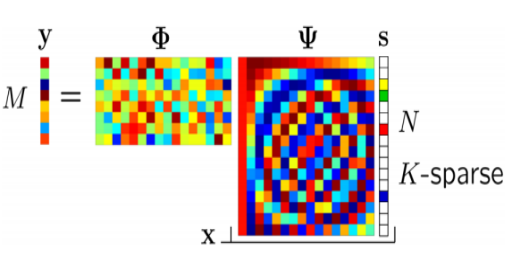
\includegraphics[scale=0.6]{CS1.png} 
\caption[A floating figure]{Measurement proces in compressed sensing.}
\label{fig:csmea} 
\end{figure}
Figure \ref{fig:csmea} depicts the operation. Putting everything together each meaasurement $y_i$ is an $ M \times 1$ vector and $\{\phi\}_{i}^{T}$ representing the rows as a $ M \times N$ matrix $\mathbf{\Phi)}$, then the sampling process is
\begin{equation} \label{eq:signal2}
\hspace{3em} \hspace{3em} \hspace{3em} y = \Phi x = \Phi\Psi\alpha \hspace{3em}
\end{equation}    
from that one can see that the product of matrices $\Phi\Psi$ has size $ M \times N$ and the measurement matrix $\mathbf{\Phi}$ in independent from the signal $\mathbf{x)}$. The previous is imporantat since the choice of the sensing matrix plays an important role for the reconstruction process, that is recovering $\mathbf{x)}$ from measurements $\mathbf{y)}$. In particular, $\Phi$ and $\Psi$ should be incoherent. Coherence of two matrices is a measure that asserts the level of correlation of $\Phi$ and $\Psi$ and is computed as follows
\begin{equation} \label{eq:signal2}
\hspace{3em} \hspace{3em} \hspace{3em} \mu(\Phi,\Psi) = \max_{k,j}|<\phi_k,\psi_j>|  \hspace{3em}
\end{equation}   
the lower $\mu$ the more incoherent the matrices are and therefore it is more probable the sucessful reconstruction of the original signal.

\subsection{Sensing matrix and RIP}
The sensing matrix $\Phi$ should be chosen so that the recons

\subsection{Signal Recovery}
   
\section{Deep Learning}

\section{Convolutional Neural Networks}

